\documentclass{UCF_ETD}
% \usepackage{times} % obsolete font package
\usepackage{url,hyperref,lineno,microtype,subcaption}
\usepackage{datetime, fmtcount, etoolbox, fcprefix}
\usepackage[T1]{fontenc}
\usepackage[utf8]{inputenc}
\usepackage{mathptmx}
\usepackage{graphicx}
\usepackage{amsmath,amssymb,amsfonts}
\usepackage{algorithmic}
\usepackage{textcomp}
\usepackage{cite}
\usepackage{graphics}
\usepackage{color,soul}
\usepackage{multirow,makecell}
\usepackage{pdfpages}
% \usepackage[backend=biber,style=numeric]{biblatex}    
% %Use absolute paths to .bib-files for the subfiles to understand their location:
\usepackage{float}
\usepackage{chapterbib}
\usepackage{subfiles}
\newcommand{\ignore}[1]{}
\newcommand{\tss}[1]{\textsuperscript{#1}}
\renewcommand{\ul}{}
\newcommand{\tsu}[1]{\textsubscript{#1}}
\newcommand{\td}{\textasciitilde}
\newcommand{\gt}{\textgreater}
\newcommand{\mt}{\textsmall}

\title{\uppercase{Corticomuscular adaptation to mechanical perturbations in a seated locomotor task}} %Must be typed in all caps.
\author{\uppercase{Seyed Yahya Shirazi}} % typed in all caps

\prevdegreeii{B.Sc. AmirKabir University of Technology (Tehran Polytechnic), 2011}
\prevdegreei{M.Sc. AmirKabir University of Technology (Tehran Polytechnic), 2014}
% commands available for 
% \prevdegreei{ }
% \prevdegreeii{ }
% \prevdegreeiii{ }

\thesisname{dissertation}
% \thesisname prints out document type. Replace bracket text with dissertation for Ph.D students

\degreename{Doctor of Philosophy in Mechanical Engineering}
% type out degree name here.

\departmentsname{Mechanical and Aerospace Engineering}
% replace with department name if applicable.  Otherwise, do not include.

%\schoolname{Kenneth G. Dixon School of Accounting}
% replace with school name if applicable.  Otherwise, do not include.

\collegename{Engineering and Computer Science}
% replace with college name

\termname{Spring}
% replace with semester

\termyear{2021}
% replace with year. Term year is also used to generate copyright year.

\advisorname{Helen J. Huang}
% replace with Major Professor if applicable.  Otherwise, do not include.


\begin{document}

\frontmatter
% applies roman numerals as page numbers

\maketitle
% prints out school info as named above

\copyrightpage{~Seyed Yahya Shirazi}
% includes copyright symbol. Term year is automatically inserted before the author name.  Replace the author name with your own, but keep the tilde in place. 

\begin{abstract}
    Cortical control during walking is most pronounced when the person is perturbed. Although seated locomotor tasks such as cycling or recumbent stepping improve walking performance, the electrocortical correlates of perturbed seated tasks have not been studied in detail. The primary purpose of this research was to quantify cortical and muscular responses to mechanical perturbations during recumbent stepping. We also aimed to quantify possible differences between young and older adults' responses to perturbed stepping. A secondary aim of this research was to determine the accuracy of electroencephalography (EEG) source imaging to interpret the electrocortical findings adequately. We hypothesized that both young and older adults would adapt to the perturbations by reducing their movement errors and reducing the anterior cingulate electrocortical activity. We also hypothesized that older adults would co-contract their agonist and antagonist muscles more than young adults in response to perturbations. Such stronger co-contraction would indicate older adults would have weaker corticomuscular connectivity in response to perturbations than young adults.

    Seventeen young adults and eleven older adults completed four perturbed arms and leg stepping tasks. We perturbed the stepping with brief 200ms increased movement resistance using a controllable servomotor on our recumbent stepper. We asked subjects to step smoothly, use both arms and legs and follow the visual pacing cue set at 60 steps per minute. We recorded brain activity with high-density EEG with 128 electrodes, muscular activity with 16 electromyography (EMG) sensors, and stepping kinematics using the servomotor's encoder. We quantified temporal and spatial motor errors from the stepping kinematics data. We used a novel post-processing approach to reject noise from EEG and estimated the electrocortical sources using independent component analysis and the current dipole estimation technique. We then performed a series of time-frequency analyses on the group EEG source data. We quantified EMG co-contraction for each of the perturbed and recovery steps. Finally, we used direct Directed Transfer Fucnction to determine the corticomuscular connectivity time-locked to young and older adults' perturbations.
    
    Quantifying the accuracy of source estimation showed that recording the three-dimensional EEG electrode locations would provide accurate source estimation up to a single Brodmann area. We also found that recording the precise location of the fiducials, i.e., the anatomical landmarks used to place the EEG electrodes, is critical for a reliable source estimation process. Motor errors did not show a reduction of errors with more perturbation experience for both young and older adults. Young adults showed significant theta-band (3-8 Hz) electrocortical activity locked to the perturbations at the anterior cingulate cortex, supplementary motor areas, and posterior parietal cortex. These locked spectral fluctuations decreased with more perturbation experience for the right-side perturbations and varied with perturbation timing. Older adults showed significant electrocortical activity with a wider spread of electrocortical sources in the motor and posterior parietal cortices. Older adults demonstrated more co-contracted muscle pairs than young adults, and co-contraction did not decrease with more perturbation experience.
    
    The results show that brief perturbation during recumbent stepping does not create error-based adaptation with reduced motor errors tied to more perturbation experience. However, these perturbations cause prolonged modifications in the motor patterns even after the perturbations are removed. Modulating the perturbation timing can tune both cortical activities at specific brain areas and modify muscular co-contraction behavior in older adults.
% abstract files can be added here.  I recommend using \input over \include
\end{abstract}

\dedication{Dedicated to my love, Maryam.}
% creates vertically and horizontally centered dedication page.  If larger than a paragraph, remove the \vspace*fil commands from the dedication section in the class file.

\begin{acknowledgments}
I have been very fortunate to be surrounded by friends and mentors that were kinder, smarter, more caring, and better than me throughout my life. I am forever in their debt.

My utmost gratitude is to my parents for their unconditional support, believing in me, and their patience during the past few years of being separated.

I am grateful to my adviser, Dr. Helen J. Huang, for seeing my potentials when others did not, and for continuously helping me grow even when it was not convenient. Thanks to her, I am becoming an expert in what I dreamed of.

I want to thank the Biomechanics, Rehabilitation, and Interdisciplinary Neuroscience (BRaIN) lab members for their scientific contributions, generous help with data collection, and our good times together. I want to especially thank Jinfeng Li and Cesar Castano for their selfless support and friendship. I am honored to have such benevolent friends at BRaIN lab and forever cherish this friendship.

I greatly appreciate the constructive comments, encouragement, and continued support of my dissertation committee, Dr. Pamela K. Douglas, Dr. Qiushi Fu, and Dr. Hwan Choi.

I want to thank all my friends in Orlando. They made Orlando home to my family and me. They soon became and forever will be my sisters, brothers, friends, and my son's sweet aunts and uncles.

Finally, I thank my wife, Maryam Sarafpour, for her love, patience, supports, and smiles for this journey that we started together some eight years ago. I could not have been here without her. I also would like to thank our son, Seyed Hani, for his hugs, laughs, and watching dad, for the past year, working from home.
\end{acknowledgments}

\tableofcontents

\listoffigures

\listoftables

\mainmatter
% restarts page numbering with arabic numbers

\subfileinclude{chapters/chap0}

\subfileinclude{chapters/chap1}

\subfileinclude{chapters/chap2}

\subfileinclude{chapters/chap3}

\subfileinclude{chapters/chap4}

\subfileinclude{chapters/chap5}

\appendix

\chapter{IRB DOCUMENTS}
\newpage
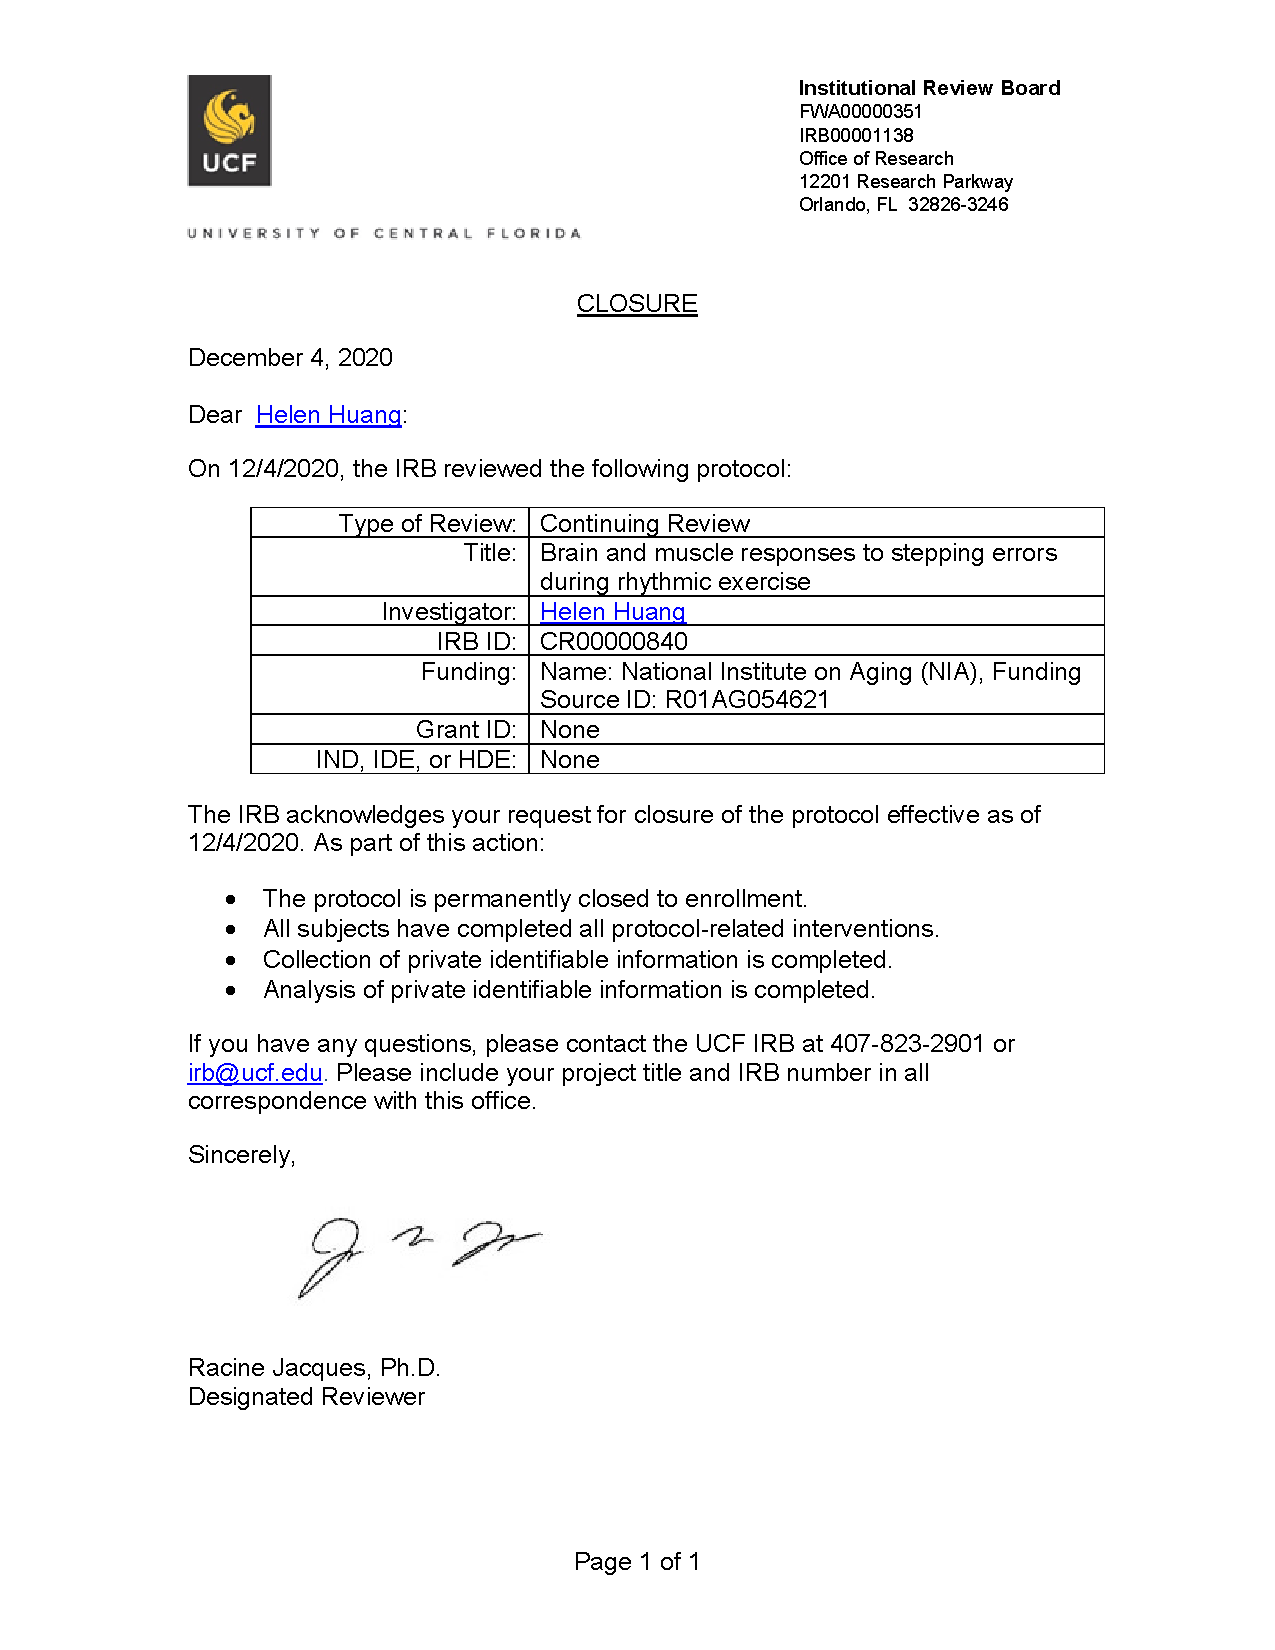
\includepdf[pages=-,scale=.8,pagecommand={}]{img/IRB approval and closure.pdf}
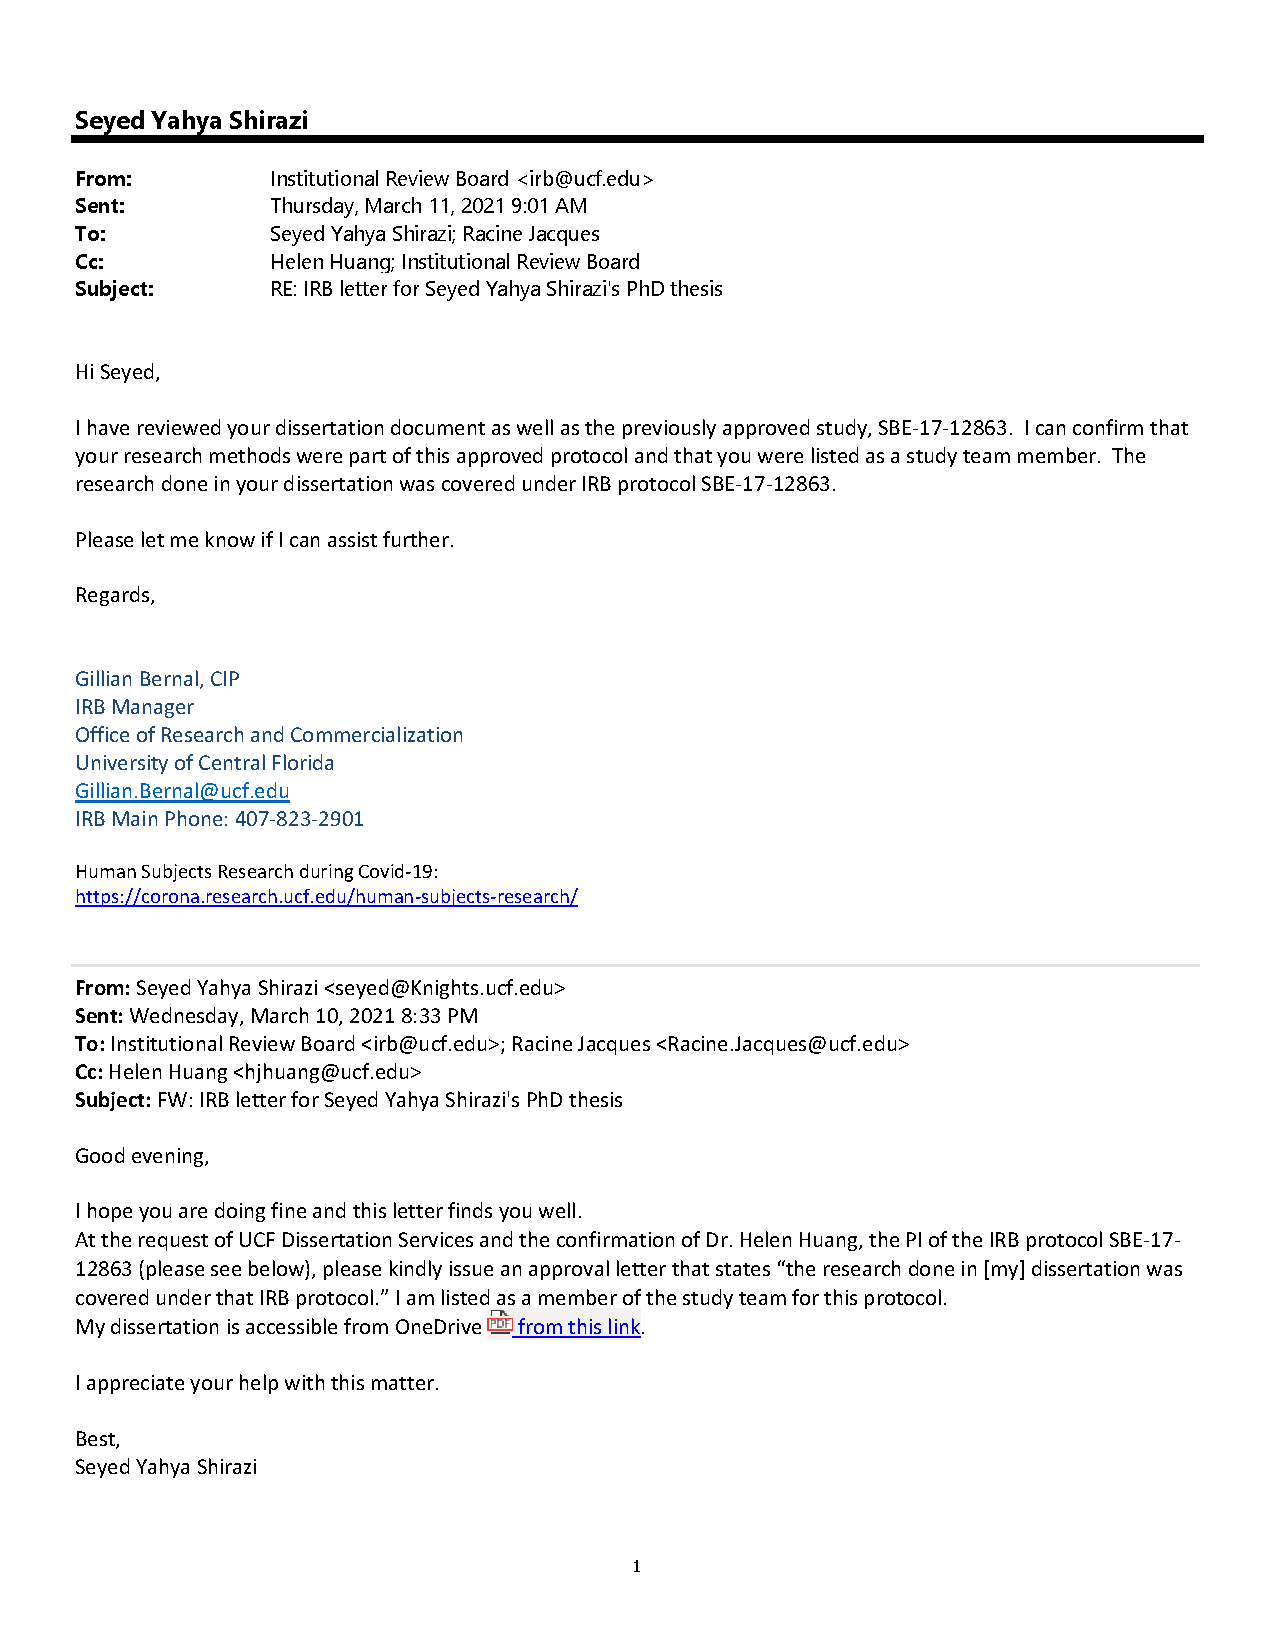
\includepdf[pages=-,scale=.8,pagecommand={}]{img/IRB approval.pdf}


\chapter{COPYRIGHT PERMISSION LETTERS}
\newpage
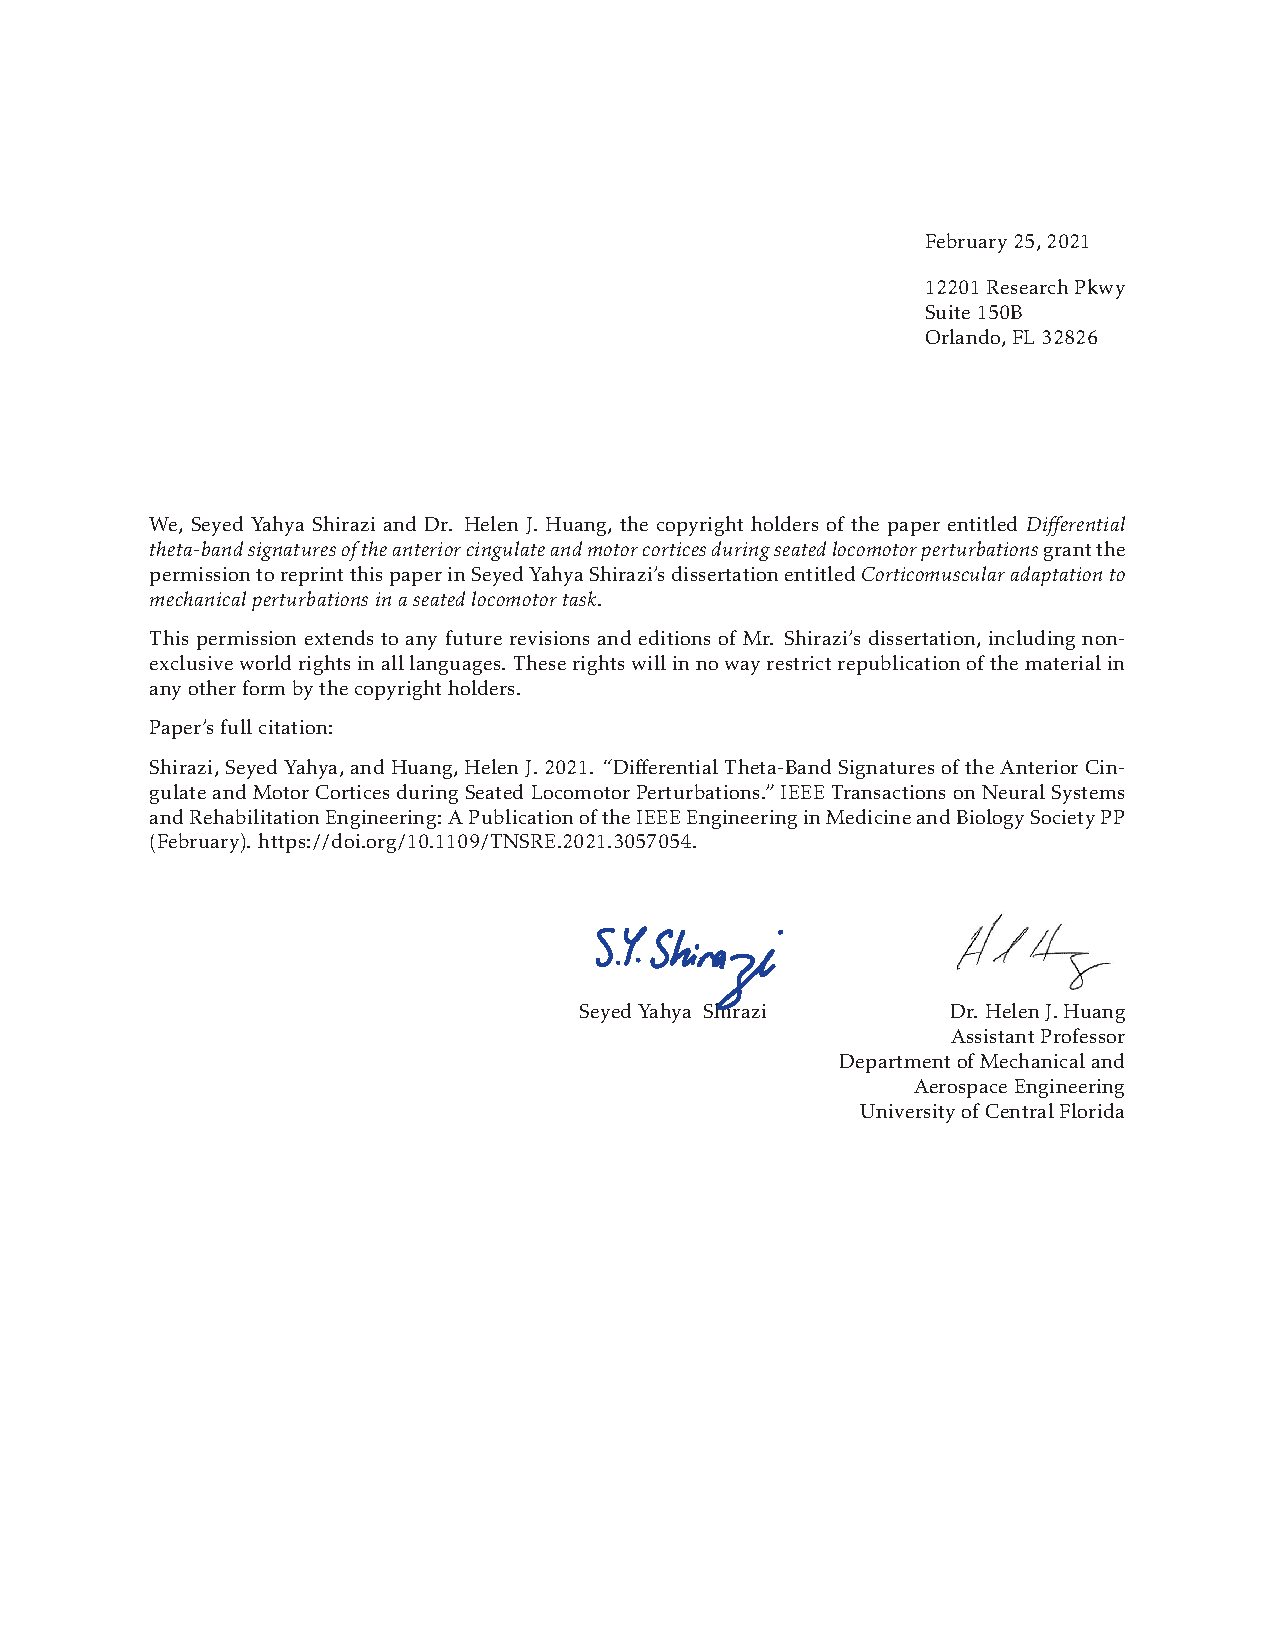
\includepdf[pages=-,scale=.8,pagecommand={}]{img/copyright authorization letters_signed-seyed-hjh_print.pdf}

\backmatter


\end{document}